\documentclass{article}
\usepackage{amsmath}
\usepackage{graphicx}
\usepackage{MnSymbol}

\begin{document}


\title{Question 38}
\author{Ana Bhattacharjee}
\date{\today}
\maketitle{}


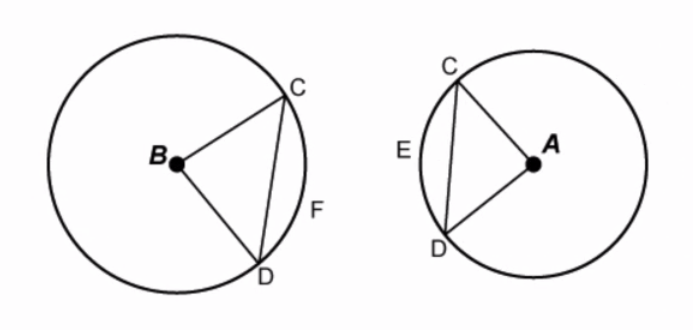
\includegraphics[width=0.9\columnwidth]{q38.png}
\paragraph{Of segments CFD and CED, which of the segments has a greater area based on the given information? Justify with your work.}
\par

\textbf{Circle A Information: }
\par
$ r = 10 m $, $ m\angle{CAD} = 90^\circ$
\par
\textbf{Circle B Information: }
\par
$ r = 12 m $, $ m\angle{CBD} = 60^\circ$

The first step is to find the area of $ \downslice CD $ for both $ \circ B $ and $ \circ A $ .

\begin{align}
  A_{\circ B} = \pi (12)^2 = 144 \pi \\
  A_{\downslice CD_{\circ B}} = \frac{60}{360} A_{\circ B} = \frac{1}{6} 144 \pi \\
  A_{\circ A} = \pi (10)^2 = 100 \pi \\
  A_{\downslice CD_{\circ A}} = \frac{90}{360} A_{\circ A} = \frac{1}{4} 100 \pi
\end{align}

\par

The next step would be to find the area of $ \triangledown{CBD} $ and $ \triangledown{CAD} $ .


\end{document}
